\documentclass{article}
\usepackage{ctex}
\usepackage{graphicx}
\usepackage{float}
\usepackage{listings}
\usepackage{xcolor}
\usepackage{caption}
\usepackage{amssymb}
\usepackage{amsmath}
\usepackage{courier}

\lstset{
    columns=fixed,       
    % numbers=left,  % 在左侧显示行号
    % numberstyle=\tiny\color{gray},   % 设定行号格式
    frame=none,                      % 不显示背景边框
    backgroundcolor=\color[RGB]{245,245,244}, % 设定背景颜色
    basicstyle=\ttfamily,
    showstringspaces=false,   % 不显示字符串中的空格
    linewidth=14cm,
}

\title{\fontsize{18}\baselineskip PA1-B Report}
\author{\fontsize{10} \baselineskip 王琛, 计65, 2016011360}
\date{}
\setlength\parindent{0pt} %default no indent

\begin{document}
\maketitle
使用的JDK版本为java version "1.8.0\_191"

\section{本阶段工作}
\subsection{错误恢复}
使用的方法和README中的相同,遇到非终结符$A$,若当前输入符号$a \notin Begin(A)$,则报错并继续往下扫描。若遇到了$Begin(A)$,恢复分析$A$,若遇到了$End(A)$,返回null并继续分析后面的符号。这部分需要注意的是执行act函数之前需要先检查params数组是否有为空的元素,如果有直接返回null,否则会产生语法错误。

\subsection{新特性的LL(1)文法}
\begin{itemize}
    \item 对象复制语句:题中的文法即是LL(1)文法,直接实现即可。
    \item 引入关键词\textmd{sealed}:题中的文法即是LL(1)文法,直接实现即可。
    \item 串行条件卫士语句:文法中开头的IF和原来IfStmt产生式左侧的IF为左公因子,需要先提取。另外,在产生IfBranch* IfSubStmt时,需要注意左递归的问题,应将左递归的因子放入产生式的右边。
    \item 简单的自动类型推导:因为var关键字,没有左公因子和左递归,直接实现即可。
    \item 若干与一维数组有关的表达式和语句:
        \begin{itemize}
            \item 数组常量:主要问题还是左递归,将递归因子放在右边即可
            \item 数组初始化常量表达式:实现方法和+、-基本相同,由于优先级低于+、-,将其放在加减前面,其余部分实现完全相同。
            \item 数组拼接表达式:同样是一个运算符,实现方法和\%\%也基本相同,由于其优先级低于\%\%,将其置于\%\%之前。唯一区别在于右递归的实现,我的思路是:和上一步的顺序遍历相反,将svec倒过来遍历,将当前元素作为第一个参数,上一步得到的expr作为第二个参数进行构造。
            \item 取子数组表达式 \&\& 数组动态下标访问表达式:这两个特性需要同时实现。原因在于两者有左公因子"[ Expr",另外为了在上一级区分两个不同的情况,在Semvalue中添加expr2,expr1用于Expr,expr2用于default Expr部分,判断两种情况是用expr1 == null 或 expr2 == null即可。
            \item python风格的comprehension表达式:由于使用新增的[|和|],文法直接是LL(1),实现即可。
            \item 数组迭代语句:本身是LL(1)文法,直接实现。
        \end{itemize}
\end{itemize}

\subsection{运行截图}
\begin{figure}[H]
    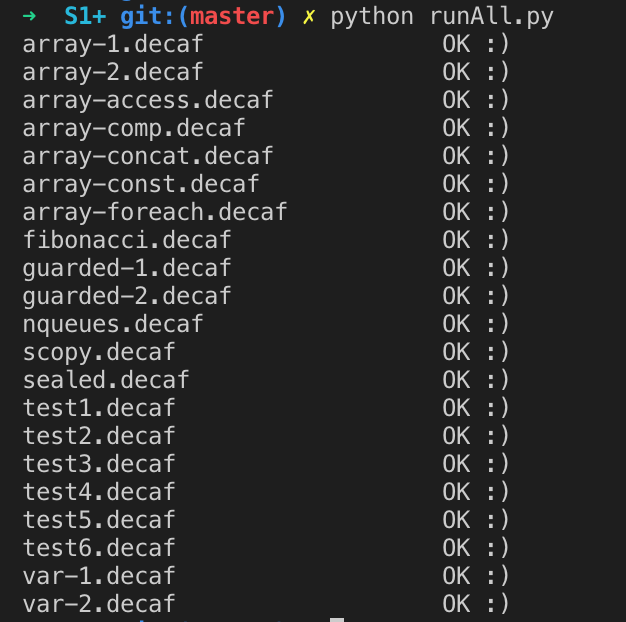
\includegraphics[width=0.60\textwidth]{1.png}
    \caption{S1+}
\end{figure}

\begin{figure}[H]
    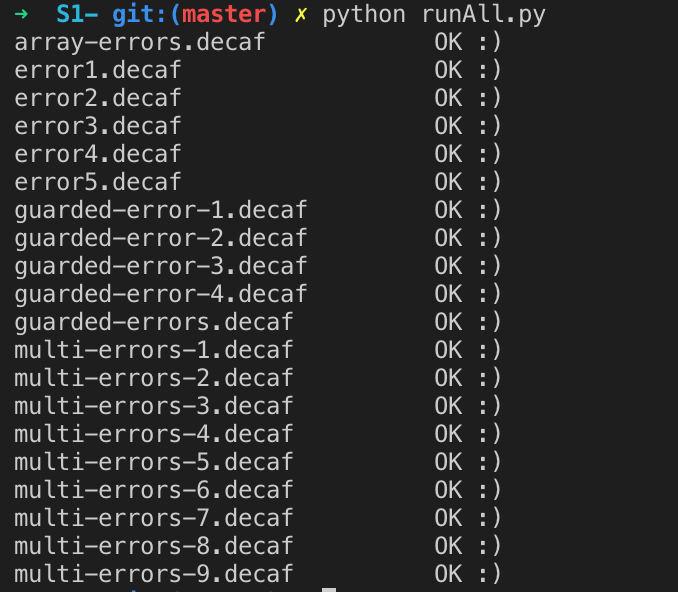
\includegraphics[width=0.60\textwidth]{2.png}
    \caption{S1-}
\end{figure}

\section{Decaf语言由于允许if语句的else分支为空,因此不是严格的 LL(1)语言,但是我 们的工具依然可以处理这种冲突。请根据工具所生成的预测分析表中if语句相关项的预测 集合先做猜测,并对照工具wiki,理解本工具的处理方法。请在实验报告中说明此方法的原理,并举一个具有这种冲突的Decaf语言程序片段,说明它哪里有冲突以及如何解决。}
实验工具是通过定义不同产生式的优先级来解决这个问题的。LL(1)的文法要求为对于每个非终结符A的任意两个产生式,$A \rightarrow \alpha$和$A \rightarrow \beta$,都有$PS(A \rightarrow \alpha) \cap PS(A \rightarrow \beta) = \varnothing$,但是由于允许if语句else为空,这个条件不再成立。令$C = PS(A \rightarrow \alpha) \cap PS(A \rightarrow \beta) = {'('}$,将$PS(A \rightarrow \beta)$改成$PS(A \rightarrow beta) - C$就满足了LL(1)文法的条件。

下面是Decaf语言中if二义性的例子:
\begin{lstlisting}
class Main {
    static void main() {
        int t;
        t = 0;
        if (t > 0) 
        if (t < 0) t = -1;
        else t = 1;
    }
}
\end{lstlisting}
若不加任何处理,else不知道会匹配到哪个if,但是利用上面的方法,匹配第一个if时无else,将会使用空,到下面的if才会匹配到else,语法分析树的结果如下。

\begin{lstlisting}
    program
    class Main <empty>
        static func main voidtype
            formals
            stmtblock
                vardef t inttype
                assign
                    varref t
                    intconst 0
                if
                    gtr
                        varref t
                        intconst 0
                    if
                        les
                            varref t
                            intconst 0
                        assign
                            varref t
                            neg
                                intconst 1
                    else
                        assign
                            varref t
                            intconst 1
\end{lstlisting}

\section{为什么把原先的数组comprehension表达式文法Expr ::= [Expr for identifier in Expr <if BoolExpr>] | ...改写为LL(1)比较困难?􏰀}
原因在于左公因子,直接使用'['和']'后产生的报错信息如下:
\begin{lstlisting}
    1 table generation:
     [java] Warning: conflict productions at line 973:
     [java] ElseClause -> ELSE Stmt
     [java] ElseClause -> <empty>
     [java] Warning: conflict productions at line 411:
     [java] Expr -> Expr1
     [java] Expr -> '[' Expr FOR IDENTIFIER IN Expr IF Expr ']'
     [java] Warning: unreachable production:
     [java] Expr -> '[' Expr FOR IDENTIFIER IN Expr IF Expr ']'
     [java] predictive set is empty
\end{lstlisting}
'['和后面数组常量的'['产生了冲突,并且这个左公因子是无法直接提出的。Parser.spec中为了确定优先级是通过逐层递进的方法,由Expr1、Expr2...越到下面优先级越高,而数组常量位于Expr9,层级相差较多,如果要消除左公因子会比较麻烦。

\section{无论何种错误处理方法,都无法完全避免误报的问题。请举出一个语法错误的Decaf程序例子,用你实现的Parser进行语法分析会带来误报。根据你用的错误处理方法,这些误报为什么会产生?}
误报程序和结果如下:
\begin{lstlisting}
    class Main {
    static void main() {
        int[] x;
        x = new int[11];
        int y;
        y = x[)10];
    }
}

*** Error at (6,15): syntax error
*** Error at (6,18): syntax error
\end{lstlisting}
第6行多了一个')',在匹配[,]中的expr时,首先遇到')'匹配失败报错,由于$) \in End(Expr)$,Expr返回null,即放弃匹配Expr, 继续向后匹配,但是对于'['放弃Expr应该匹配']',这时却出现10了,因此再次报错。实际上,应该只报'('的错,这里却产生了误报。

\section*{Acknowledgement}
本次实验李映辉同学曾给予我思路的指导,尤其是数组拼接表达式和数组动态下标访问的实现。
\end{document}
    